% ============================================================================================
% ======= On force le passage des options au paquet xcolor pour l'utilisation
% ======= du paquet profcollege
% ============================================================================================
\PassOptionsToPackage{table}{xcolor}
\PassOptionsToPackage{svgnames}{xcolor}
\documentclass[nocrop]{sesamanuel}
% ============================================================================================
% ======= Générer les correction dans un dossier spécifique
% ============================================================================================

\renewcommand\PrefixeCorrection{corrections/}
% ============================================================================================
% ======= Thèmes de base prédéfinis
% \themaG ; \themaF ; \themaS
%
% ======= Thèmes personnalisés
%
% \NewThema{N}{n}{titre}{Titre}{TITRE}{couleur entete et ...}{couleur pied de page et ...}
%
% ============================================================================================
\NewThema{N}{n}{nombres \&\\~calculs}{Nombres \&\\~calculs}{NOMBRES \&\\~CALCULS}{B1}{B1!50}

% Pour la géométrie on garde le théme d'origine

\NewThema{D}{d}{organisation \&\\~gestion de données}{Organisation \&\\~gestion de données}{ORGANISATION \&\\~GESTION DE DONNÉES}{PartieStatistique}{PartieStatistique!50}

\NewThema{M}{m}{grandeurs \&\\~mesures}{Grandeurs \&\\~mesures}{GRANDEURS \&\\~MESURES}{G1}{G1!50}

\NewThema{A}{a}{algorithmique \&\\~programmation}{Algorithmique \&\\~programmation}{ALGORITHMIQUE \&\\~PROGRAMMATION}{J1}{J1!50}

% ============================================================================================
% ======= Comme il y a des thèmes personnalisés
% ======= Il faut redefinir la commande \ListeMethodesThemes{}
% ============================================================================================

\renewcommand\ListeMethodesThemes{{n}{N},{d}{D},{g}{G},{m}{M},{a}{A}}
% ============================================================================================
\usepackage{sesamanuelTIKZ}
\usepackage{ProfCollege}
% Pour la gestion des fontes.
\usepackage{unicode-math}
% Par exemple, une fonte sans serif pour les briques Scratch.
\newfontfamily\myfontScratch[]{FreeSans}

\begin{document}

% ============================================================================================
% ======= Tests
% ============================================================================================

\themaN
\chapter{themaN1}
% ============================================================================================
% ======= Rappels de connaissances et série de petits exercices
% ============================================================================================

\begin{prerequis}
    Liste de prérequiss - Ici le tritre est le titre par défaut
    \begin{itemize}
    \item prérequis 1
    \item prérequis 2
    \item prérequis 3
    \item prérequis 4    
    \end{itemize}
\end{prerequis}

\begin{prerequis}[Titre prérequis modifié]
    Liste de prérequis - Ici le tritre est modifié
    \begin{itemize}
    \item prérequis 1
    \item prérequis 2
    \item prérequis 3
    \item prérequis 4    
    \end{itemize}
\end{prerequis}


\begin{autoeval}
    \begin{multicols}{2}
      \begin{exercice}
        Ex1
      \end{exercice}
      \begin{corrige}
        corEx1
      \end{corrige}
      \begin{exercice}
        Ex2
      \end{exercice}
      \begin{corrige}
        corEx2
      \end{corrige}
  \vfill \columnbreak
      \begin{exercice}
        Ex3
      \end{exercice}
      \begin{corrige}
        corEx3
      \end{corrige}
    \end{multicols}
  \end{autoeval}

  \cours  
  \begin{methode}[Titre de la méthode chapN1]
    Texte introductif
    \exercice
    Texte de l’exercice
    \correction
    Texte de la correction sur un minimum de trois lignes pour faire la
    différence entre vis-à-vis et double colonne. C’est l’endroit de la
    coupure qui va différer.
  \end{methode}
  
  \begin{methode*1}[Titre de la méthode*1  chapN1]
    Texte introductif
    \exercice
    Texte de l’exercice
    \correction
    Texte de la correction sur un minimum de trois lignes pour faire la
    différence entre vis-à-vis et double colonne. C’est l’endroit de la
    coupure qui va différer.
  \end{methode*1}
  
  \begin{methode*2}[Titre de la méthode*2  chapN1]
    Texte introductif
    \exercice
    Texte de l’exercice
    \correction
    Texte de la correction sur un minimum de trois lignes pour faire la
    différence entre vis-à-vis et double colonne. C’est l’endroit de la
    coupure qui va différer.
  \end{methode*2}
  
  \begin{methode*2*2}[Dernière méthode  chapN1]
    \exercice    
    Texte du premier exercice
    \correction
    Correction du premier exercice
    \exercice
    Texte du deuxième exercice
    \correction
    Texte de la correction du deuxième exercice sur un minimum de trois
    lignes pour faire la différence entre vis-à-vis et double
    colonne. C’est l’endroit de la coupure qui va différer.
  \end{methode*2*2}

% ============================================================================================
% ======= Rappels de connaissances et série de petits exercices avec ProfCollege
% ============================================================================================

\chapter{themaN2}

\begin{prerequis}[Tables de multiplication]
    Premier test d'inclusion de commandes du paquet \textbf{profcollege}
    \begin{itemize}
    \item La commande \textbackslash defiTable{}
    \item La commande \textbackslash defiTableText{}
    \end{itemize}
\end{prerequis}


\begin{autoeval}
      \begin{exercice}
        \DefiTable{%
            - x ç w j è , k ö $:$%ligne 1
            §w è k $:$ a q \og{} r l%ligne 2
            §ô a g r d m f t%ligne 3
            §\og{} l m b é o c%ligne 4
            §s t à c . ê%ligne 5
            §o e i p z%ligne 6
            §h u ' y%ligne 7
            §n v î%ligne 8
            §\fg{} â%ligne 9
            §!%ligne 10
        }
        \par 
        \DefiTableTexte{%
            14/56/12/64/21/*/30/56/*/12/56/18/12/25%ligne 1
            §27/48/64/48/7/*/21/42/25/25/48/64/42/*/56/64%ligne 2
            §40/36/42/56/18/*/12/56/*/30/12/28/20/42/12/56/45%
            }{%
            quand*tu*auras
            §fini,*dessine*un
            §coeur*au*tableau.
        }
      \end{exercice}
      \begin{corrige}
        \DefiTableTexte[Solution]{%
            14/56/12/64/21/*/30/56/*/12/56/18/12/25%ligne 1
            §27/48/64/48/7/*/21/42/25/25/48/64/42/*/56/64%ligne 2
            §40/36/42/56/18/*/12/56/*/30/12/28/20/42/12/56/45%
            }{%
            quand*tu*auras
            §fini,*dessine*un
            §coeur*au*tableau.
        }
      \end{corrige}
      \begin{exercice}
        Ex2
      \end{exercice}
      \begin{corrige}
        corEx2
      \end{corrige}
      \begin{exercice}
        Ex3
      \end{exercice}
      \begin{corrige}
        corEx3
      \end{corrige}
  \end{autoeval}

  \cours  
  \begin{methode}[Titre de la méthode chapN2]
    Texte introductif
    \exercice
    Texte de l’exercice
    \correction
    Texte de la correction sur un minimum de trois lignes pour faire la
    différence entre vis-à-vis et double colonne. C’est l’endroit de la
    coupure qui va différer.
  \end{methode}

\themaD

% ============================================================================================
% ======= Rappels + petits exercices + Activités d'approche
% ============================================================================================

\chapter{themaD1}
\begin{prerequis}[Prérequis - D1]
  Chapitre avec Rappels, petits exercices
  \begin{itemize}
  \item Rappels
  \item Petits exercices
  \end{itemize}
\end{prerequis}

\begin{autoeval}
  \begin{multicols}{2}
    \begin{exercice}
      Ex1
    \end{exercice}
    \begin{corrige}
      corEx1
    \end{corrige}
    \begin{exercice}
      Ex2
    \end{exercice}
    \begin{corrige}
      corEx2
    \end{corrige}
\vfill \columnbreak
    \begin{exercice}
      Ex3
    \end{exercice}
    \begin{corrige}
      corEx3
    \end{corrige}
  \end{multicols}
\end{autoeval}

% ============================================================================================
% ======= Activités d'approche
% ======= \tice et \logo sont les deux seuls logos disponibles
% ======= On peut éventuellement reprendre la structure des commandes pour en définir d'autres
% ============================================================================================

  \activites
  \begin{activite}[Titre de l’activité][\tice]
  Texte de l’activité... Avec titre et logo
  \end{activite}
  \begin{debat}[Titre du débat][\algo]
  Texte du débat... Avec titre et logo
  \end{debat}
  \begin{activite}[Titre de l’activité]
  Texte de l’activité... sans logo
  \end{activite}
  \begin{debat}
  Texte du débat... Sans titre ni logo
  \end{debat}
  \DeclareActivityLike{nouveau}{DÉCOUVERTE}{lime}{orange}{red}
  \begin{nouveau}[titre][\tice]
  Un nouvel environnement de type activité...

  Fonctionnement identique.
  \end{nouveau}


  \cours  
  \begin{methode}[Titre de la méthode chapD1]
    Texte introductif
    \exercice
    Texte de l’exercice
    \correction
    Texte de la correction sur un minimum de trois lignes pour faire la
    différence entre vis-à-vis et double colonne. C’est l’endroit de la
    coupure qui va différer.
  \end{methode}

%\chapter{themaD2}

\themaG
% ============================================================================================
% ======= Chapitre témoin complet
% ======= Rappels + petits exercices + Activités d'approche + cours et commandes 
% ======= Recreation/Enigme + Tests + Travaux Pratiques
% ============================================================================================

\chapter{themaG1}
\begin{prerequis}[Prérequis - G1]
  Chapitre avec Rappels, petits exercices, activités/débats
  \begin{itemize}
  \item Rappels
  \item Petits exercices
  \item Activités
  \item Débats
  \item ActivityLike
  \end{itemize}
\end{prerequis}

\begin{autoeval}  
    \begin{exercice}
      Ex1
    \end{exercice}
    \begin{corrige}
      G1-corEx1
    \end{corrige}
    \begin{exercice}
      Ex2
    \end{exercice}
    \begin{corrige}
      G1-corEx2
    \end{corrige}
\end{autoeval}

\activites
\begin{activite}[Titre de l’activité][\tice]
  Texte de l’activité... Avec titre et logo
\end{activite}
\begin{debat}[Titre du débat][\algo]
  Texte du débat... Avec titre et logo
\end{debat}

\cours
\section{Section 1}
\subsection{Sous-section 1.1}
\begin{definition}[Titre optionnel]
  Dans le cours, on utilise assez souvent des cadres du type
  définition (comme ici par exemple).
\end{definition}
\begin{remarque}
  Ceci est une remarque.
\end{remarque}
\begin{propriete}[Titre optionnel]
  Dans le cours, on utilise assez souvent des cadres du type
  définition, comme ici par exemple pour une propriete.
\end{propriete}
\begin{remarques}
  \begin{itemize}
    \item remarque.
    \item remarque.
  \end{itemize}
\end{remarques}
\begin{theoreme}[Titre optionnel]
  Dans le cours, on utilise assez souvent des cadres du type
  définition, comme ici par exemple pour un théorème.
\end{theoreme}
\begin{notation}
  notation
\end{notation}
\begin{notations}
  \begin{itemize}
    \item notation.
    \item notation.
  \end{itemize}
\end{notations}
\begin{preuve}
  Ceci est une preuve\par Deuxième ligne de la preuve
\end{preuve}
\begin{exemple}
  Texte de l’exemple
  \correction
  Texte de la correction en vis à vis
\end{exemple}

\begin{exemple*1}
  Texte de l’exemple
  \correction
  Texte de la correction, le tout verticalement affiché
\end{exemple*1}

\begin{exemple}[0.6]
  Texte de l’exemple très long sur une ligne, très très très long.
  On peut modifier la répartition horizontale  à l'aide d'un argument optionnel valant par défaut 0,4, valant ici 0,6.
  \correction
  Texte de la correction en vis à vis
\end{exemple}

\subsection{Sous-section 1.2}
Quatre affichages prévus pour les méthodes.

\begin{methode}[Titre de la méthode chapG1]
  Texte introductif
  \exercice
  Texte de l’exercice
  \correction
  Texte de la correction sur un minimum de trois lignes pour faire la
  différence entre vis-à-vis et double colonne. C’est l’endroit de la
  coupure qui va différer.
\end{methode}

\begin{methode*1}[Titre de la méthode*1 chapG1]
  Texte introductif
  \exercice
  Texte de l’exercice
  \correction
  Texte de la correction sur un minimum de trois lignes pour faire la
  différence entre vis-à-vis et double colonne. C’est l’endroit de la
  coupure qui va différer.
\end{methode*1}

\begin{methode*2}[Titre de la méthode*2 chapG1]
  Texte introductif
  \exercice
  Texte de l’exercice
  \correction
  Texte de la correction sur un minimum de trois lignes pour faire la
  différence entre vis-à-vis et double colonne. C’est l’endroit de la
  coupure qui va différer.
\end{methode*2}

\begin{methode*2*2}[Dernière méthode  chapG1\MethodeRefExercice{exo-exemple1} \MethodeRefExercice{exo-exemple2}]
  \exercice
  \label{methode-exemple}
  Texte du premier exercice
  \correction
  Correction du premier exercice
  \exercice
  Texte du deuxième exercice
  \correction
  Texte de la correction du deuxième exercice sur un minimum de trois
  lignes pour faire la différence entre vis-à-vis et double
  colonne. C’est l’endroit de la coupure qui va différer.
\end{methode*2*2}

\section{Section 2}
Texte Section 2
\subsection{Sous-section 2.1}
Texte Sous-section 2.1
\subsection{Sous-section 2.2}
Texte Sous-section 2.1

\exercicesbase
\begin{colonne*exercice}
  \serie{titre de série1}
  \begin{exercice}[Exercice sans correction][\tice]
  Prouver que $1=1$
  \end{exercice}
  \begin{exercice*}[Exercice* avec correction]
  Prouver que $2=2$
  \end{exercice*}
  \begin{corrige}
  On sait que $1=1$ avec l’exercice précédent donc $1+1=1+1$,
  c’est-à-dire $2=2$.
  \end{corrige}
  \begin{exercice}[Lien avec une méthode \ExerciceRefMethode{methode-exemple}]
  \label{exo-exemple1}
  Test pour avoir un lien avec une méthode.
  \end{exercice}
  \begin{exercice}[Exercice sans correction][\algo]
    Prouver que $7=7$
  \end{exercice}

  \serie{titre de série2}
  \begin{exercice}[Exercice sans correction][\tice]
    \partie
    Prouver que $1=1$
    \partie
    En déduire que $2=2$
    \partie 
    Puis que $3=3$
  \end{exercice}
  \begin{exercice*}[Exercice* avec correction]
  Prouver que $2=2$
  \end{exercice*}
  \begin{corrige}
  On sait que $1=1$ avec l’exercice précédent donc $1+1=1+1$,
  c’est-à-dire $2=2$.
  \end{corrige}
\end{colonne*exercice}

\exercicesappr
\begin{colonne*exercice}
  \serie{titre de série1}
  \begin{exercice}[Exercice sans correction][\tice]
  Prouver que $1=1$
  \end{exercice}
  \begin{exercice*}[Exercice* avec correction]
  Prouver que $2=2$
  \end{exercice*}
  \begin{corrige}
  On sait que $1=1$ avec l’exercice précédent donc $1+1=1+1$,
  c’est-à-dire $2=2$.
  \end{corrige}
  \begin{exercice}[Lien avec une méthode \ExerciceRefMethode{methode-exemple}]
  \label{exo-exemple2}
  Test pour avoir un lien avec une méthode.
  \end{exercice}
  \begin{exercice}[Exercice sans correction][\algo]
    Prouver que $7=7$
  \end{exercice}

  \serie{titre de série2}
  \begin{exercice}[Exercice sans correction][\tice]
    \partie
    Prouver que $1=1$
    \partie
    En déduire que $2=2$
    \partie 
    Puis que $3=3$
  \end{exercice}
  \begin{exercice*}[Exercice* avec correction]
  Prouver que $2=2$
  \end{exercice*}
  \begin{corrige}
  On sait que $1=1$ avec l’exercice précédent donc $1+1=1+1$,
  c’est-à-dire $2=2$.
  \end{corrige}
\end{colonne*exercice}

% La commande \Recreation permet d'inclure un saut de page

\recreation
\begin{enigme}
  Trouveras-tu un chemin de multiples entre les cases colorées ?
  \par
  \LabyNombre[Multiple=7,Longueur=12,Largeur=8,XDepart=2,YDepart=2,XArrivee=11,YArrivee=6,Murs]
\end{enigme}

% ============================================================================================
% ======= Je teste mes connaissances
% ============================================================================================

\connaissances
\begin{acquis}
\begin{itemize}
\item Premier point à connaître.
\item Autre point à savoir faire.
\item Dernier point devant être su.
\end{itemize}
\end{acquis}

\QCMautoevaluation{texte introductif}

\begin{QCM}
  \begin{EnonceCommunQCM}
    Pour les questions \RefQCM{premier-qcm} à
    \RefQCM{deuxieme-qcm}, $f$ désigne une
    fonction affine.
    \end{EnonceCommunQCM}

\begin{GroupeQCM}
\begin{exercice}\label{premier-qcm}
La courbe de $f$ est
\begin{ChoixQCM}{3}
\item une droite
\item une parabole
\item autre
\end{ChoixQCM}
\end{exercice}
\begin{corrige}
\reponseQCM{a}
\end{corrige}
\begin{exercice}\label{deuxieme-qcm}
$f(3)$
\begin{ChoixQCM}{3}
\item vaut la moitié de $f(6)$
\item vaut le double de $f(6)$
\item on ne peut pas savoir
\end{ChoixQCM}
\end{exercice}
\begin{corrige}
\reponseQCM{c}
\end{corrige}
\end{GroupeQCM}
\end{QCM}

\TravauxPratiques
\begin{TP}[Titre Optionnel][\tice]
  Contenu TP
  \partie{Titre partie 1}
  
  TP partie 1
  
  \partie{Titre partie 2}
  
  TP partie 2
  
  \partie{Titre partie 3}
  
  TP partie 3 
\end{TP}

\recreation
  \begin{enigme}[Titre optionnel]
    Enigme/Recreation

    Scratch avec profcollege

      \begin{Scratch}
        Place Drapeau;
        Place Avancer("50");
        Place Repeter("10");
        Place Tournerg("36");
        Place Avancer("50");
        Place FinBlocRepeter;
        \end{Scratch}

    \end{enigme}

% ============================================================================================
% ======= Annexes
% ======= Interdictions a priori
% ==========> L'environnement "corrige" --> Il semble que non
% ==========> La commande \partie en dehors d'un exercice
%
% ======= On peut changer les couleurs des annexes avec \ChangeAnnexe{}{}{}{}
% ======= Attention il faut mettre cette commande avant le premier appel à \annexe{}
% ======= sinon ça change toutes les annexes sauf la première !
% ======= L'appel par défaut est \ChangeAnnexe{G3}{A1}{G1}{Blanc}
% ============================================================================================
\ChangeAnnexe{J3}{H1}{J1}{Blanc}
\annexe{Titre annexe I}

\begin{prerequis}[Prérequis - G1]
  Chapitre avec Rappels, petits exercices  
  \begin{itemize}
  \item Rappels
  \item Petits exercices
  \end{itemize}
\end{prerequis}

\begin{autoeval}  
    \begin{exercice}
      Ex1
    \end{exercice}
    \begin{corrige}
      AnnexeI - Cor Ex1
    \end{corrige}
\end{autoeval}

\activites
\begin{activite}[Titre de l’activité][\tice]
  Texte de l’activité... Avec titre et logo
\end{activite}
\begin{debat}[Titre du débat][\algo]
  Texte du débat... Avec titre et logo
\end{debat}

\cours
\section{Section 1}
\subsection{Sous-section 1.1}
\begin{definition}[Titre optionnel]
  Dans le cours, on utilise assez souvent des cadres du type
  définition (comme ici par exemple).
\end{definition}
\begin{remarque}
  Ceci est une remarque.
\end{remarque}
\begin{propriete}[Titre optionnel]
  Dans le cours, on utilise assez souvent des cadres du type
  définition, comme ici par exemple pour une propriete.
\end{propriete}
\begin{remarques}
  \begin{itemize}
    \item remarque.
    \item remarque.
  \end{itemize}
\end{remarques}
\begin{theoreme}[Titre optionnel]
  Dans le cours, on utilise assez souvent des cadres du type
  définition, comme ici par exemple pour un théorème.
\end{theoreme}
\begin{notation}
  notation
\end{notation}
\begin{notations}
  \begin{itemize}
    \item notation.
    \item notation.
  \end{itemize}
\end{notations}
\begin{preuve}
  Ceci est une preuve\par Deuxième ligne de la preuve
\end{preuve}
\begin{exemple}
  Texte de l’exemple
  \correction
  Texte de la correction en vis à vis
\end{exemple}

\begin{exemple*1}
  Texte de l’exemple
  \correction
  Texte de la correction, le tout verticalement affiché
\end{exemple*1}

\begin{exemple}[0.6]
  Texte de l’exemple très long sur une ligne, très très très long.
  On peut modifier la répartition horizontale  à l'aide d'un argument optionnel valant par défaut 0,4, valant ici 0,6.
  \correction
  Texte de la correction en vis à vis
\end{exemple}

\begin{methode}[Titre de la méthode G1-AnnexeI]
  Texte introductif
  \exercice
  Texte de l’exercice
  \correction
  Texte de la correction sur un minimum de trois lignes pour faire la
  différence entre vis-à-vis et double colonne. C’est l’endroit de la
  coupure qui va différer.
\end{methode}

\begin{methode*1}[Titre de la méthode*1 G1-AnnexeI]
  Texte introductif
  \exercice
  Texte de l’exercice
  \correction
  Texte de la correction sur un minimum de trois lignes pour faire la
  différence entre vis-à-vis et double colonne. C’est l’endroit de la
  coupure qui va différer.
\end{methode*1}

\begin{methode*2}[Titre de la méthode*2 G1-AnnexeI]
  Texte introductif
  \exercice
  Texte de l’exercice
  \correction
  Texte de la correction sur un minimum de trois lignes pour faire la
  différence entre vis-à-vis et double colonne. C’est l’endroit de la
  coupure qui va différer.
\end{methode*2}

\begin{methode*2*2}[Dernière méthode G1-AnnexeI\MethodeRefExercice{exo-exemple1} \MethodeRefExercice{exo-exemple2}]
  \exercice
  \label{methode-exemple2}
  Texte du premier exercice
  \correction
  Correction du premier exercice
  \exercice
  Texte du deuxième exercice
  \correction
  Texte de la correction du deuxième exercice sur un minimum de trois
  lignes pour faire la différence entre vis-à-vis et double
  colonne. C’est l’endroit de la coupure qui va différer.
\end{methode*2*2}

\exercicesbase
\begin{colonne*exercice}
  \serie{titre de série1}
  \begin{exercice}[Exercice sans correction][\tice]
  Prouver que $1=1$
  \end{exercice}
  \begin{exercice*}[Exercice* avec correction]
  Prouver que $2=2$
  \end{exercice*}
  \begin{corrige}
  AnnexeI -

  On sait que $1=1$ avec l’exercice précédent donc $1+1=1+1$,
  c’est-à-dire $2=2$.
  \end{corrige}
  \begin{exercice}[Lien avec une méthode \ExerciceRefMethode{methode-exemple2}]
  \label{exo-exemple3}
  Test pour avoir un lien avec une méthode.
  \end{exercice}
  \begin{exercice}[Exercice sans correction][\algo]
    Prouver que $7=7$
  \end{exercice}

  \serie{titre de série2}
  \begin{exercice}[Exercice sans correction][\tice]
    \partie
    Prouver que $1=1$
    \partie
    En déduire que $2=2$
    \partie 
    Puis que $3=3$
  \end{exercice}
  \begin{exercice*}[Exercice* avec correction]
  Prouver que $2=2$
  \end{exercice*}
  \begin{corrige}
    AnnexeI -

  On sait que $1=1$ avec l’exercice précédent donc $1+1=1+1$,
  c’est-à-dire $2=2$.
  \end{corrige}
\end{colonne*exercice}

\exercicesappr
\begin{colonne*exercice}
  \serie{titre de série1}
  \begin{exercice}[Exercice sans correction][\tice]
  Prouver que $1=1$
  \end{exercice}
  \begin{exercice*}[Exercice* avec correction]
  Prouver que $2=2$
  \end{exercice*}
  \begin{corrige}
    AnnexeI -
  On sait que $1=1$ avec l’exercice précédent donc $1+1=1+1$,
  c’est-à-dire $2=2$.
  \end{corrige}
  \begin{exercice}[Lien avec une méthode \ExerciceRefMethode{methode-exemple2}]
  \label{exo-exemple4}
  Test pour avoir un lien avec une méthode.
  \end{exercice}
  \begin{exercice}[Exercice sans correction][\algo]
    Prouver que $7=7$
  \end{exercice}

  \serie{titre de série2}
  \begin{exercice}[Exercice sans correction][\tice]
    \partie
    Prouver que $1=1$
    \partie
    En déduire que $2=2$
    \partie 
    Puis que $3=3$
  \end{exercice}
  \begin{exercice*}[Exercice* avec correction]
  Prouver que $2=2$
  \end{exercice*}
  \begin{corrige}
    AnnexeI -
  On sait que $1=1$ avec l’exercice précédent donc $1+1=1+1$,
  c’est-à-dire $2=2$.
  \end{corrige}
\end{colonne*exercice}

% La commande \Recreation permet d'inclure un saut de page

\recreation
\begin{enigme}
  Trouveras-tu un chemin de multiples entre les cases colorées ?
  \par
  \LabyNombre[Multiple=7,Longueur=12,Largeur=8,XDepart=2,YDepart=2,XArrivee=11,YArrivee=6,Murs]
\end{enigme}

% ============================================================================================
% ======= Je teste mes connaissances
% ============================================================================================

\connaissances
\begin{acquis}
\begin{itemize}
\item Premier point à connaître.
\item Autre point à savoir faire.
\item Dernier point devant être su.
\end{itemize}
\end{acquis}

\QCMautoevaluation{texte introductif}

\begin{QCM}
  \begin{EnonceCommunQCM}
    Pour les questions \RefQCM{premier-qcm} à
    \RefQCM{deuxieme-qcm}, $f$ désigne une
    fonction affine.
    \end{EnonceCommunQCM}

\begin{GroupeQCM}
\begin{exercice}\label{premier-qcm2}
La courbe de $f$ est
\begin{ChoixQCM}{3}
\item une droite
\item une parabole
\item autre
\end{ChoixQCM}
\end{exercice}
\begin{corrige}
  AnnexeI -
\reponseQCM{a}
\end{corrige}
\begin{exercice}\label{deuxieme-qcm2}
$f(3)$
\begin{ChoixQCM}{3}
\item vaut la moitié de $f(6)$
\item vaut le double de $f(6)$
\item on ne peut pas savoir
\end{ChoixQCM}
\end{exercice}
\begin{corrige}
  AnnexeI -
\reponseQCM{c}
\end{corrige}
\end{GroupeQCM}
\end{QCM}

\TravauxPratiques
\begin{TP}[Titre Optionnel][\tice]
  Contenu TP
  \partie{Titre partie 1}
  
  TP partie 1
  
  \partie{Titre partie 2}
  
  TP partie 2
  
  \partie{Titre partie 3}
  
  TP partie 3 
\end{TP}

\recreation
  \begin{enigme}[Titre optionnel]
    AnnexeI -
    
    Enigme/Recreation

    Scratch avec profcollege

      \begin{Scratch}
        Place Drapeau;
        Place Avancer("50");
        Place Repeter("10");
        Place Tournerg("36");
        Place Avancer("50");
        Place FinBlocRepeter;
        \end{Scratch}

    \end{enigme}

\annexe{Titre annexe II}
\begin{prerequis}[Prérequis - G1]
  Chapitre avec Rappels, petits exercices  
  \begin{itemize}
  \item Rappels
  \item Petits exercices
  \end{itemize}
\end{prerequis}

\begin{autoeval}  
    \begin{exercice}
      Ex1
    \end{exercice}
    \begin{corrige}
      AnnexeII -
      Cor Ex1
    \end{corrige}
    \begin{exercice}
      Ex2
    \end{exercice}
    \begin{corrige}
      AnnexeII -
      Cor Ex2
    \end{corrige}
\end{autoeval}

\annexe{Titre annexe III}

\begin{prerequis}[Prérequis - G1]
  Chapitre avec Rappels, petits exercices  
  \begin{itemize}
  \item Rappels
  \item Petits exercices
  \end{itemize}
\end{prerequis}

\begin{autoeval}  
    \begin{exercice}
      Ex1
    \end{exercice}
    \begin{corrige}
      AnnexeIII -
      Cor Ex1
    \end{corrige}
    \begin{exercice}
      Ex2
    \end{exercice}
    \begin{corrige}
      AnnexeIII -
      Cor Ex2
    \end{corrige}
\end{autoeval}

%\chapter{themaG2}
%\chapter{themaG3}

\themaM
\chapter{themaM1}
\cours  
\begin{methode}[Titre de la méthode chapM1]
  Texte introductif
  \exercice
  Texte de l’exercice
  \correction
  Texte de la correction sur un minimum de trois lignes pour faire la
  différence entre vis-à-vis et double colonne. C’est l’endroit de la
  coupure qui va différer.
\end{methode}

%\chapter{themaM2}

\themaA
\chapter{themaA1}
\cours  
\begin{methode}[Titre de la méthode chapA1]
  Texte introductif
  \exercice
  Texte de l’exercice
  \correction
  Texte de la correction sur un minimum de trois lignes pour faire la
  différence entre vis-à-vis et double colonne. C’est l’endroit de la
  coupure qui va différer.
\end{methode}

\begin{autoeval}  
  \begin{exercice}
    Ex1
  \end{exercice}
  \begin{corrige}
    Cor Ex1
  \end{corrige}
  \begin{exercice}
    Ex2
  \end{exercice}
  \begin{corrige}
    Cor Ex2
  \end{corrige}
\end{autoeval}

%\chapter{themaA2}
%\chapter{themaA3}

% ============================================================================================
% ======= Liste des méthodes
% ============================================================================================
\AfficheListeMethodes[1]

% ============================================================================================
% ======= Solutions des exercices
% ============================================================================================

\AfficheCorriges[1]

% ============================================================================================
% ======= Glossaire de propriétés
% ============================================================================================

\annexe{Titre Glossaire de propriétés}

\begin{cadre}[A1][A4] 
Glossaire
 \begin{itemize}
 \item item1
 \item item2
 \item item3
 \item item4
 \end{itemize}
 suite glossaire
\end{cadre}

\section{Section 1 \textcolor{A1}{texte en couleur différente}}
\ListeProprietes{1} à \ListeProprietes{3}
\section{Section 2 \textcolor{A1}{texte en couleur différente}}
\ListeProprietes{4} à \ListeProprietes{7}

\clearpage
\begin{tableau}[pr]{\linewidth}
  \hline %%%%%%%%%%%%%%%%%%%%%%P1 
  \begin{pspicture}(0,0.25)(3.5,2.5)
  \pnode(0,0.5){A}
  \pnode(2.5,0.5){B}
  \pnode(3.5,2){C}
  \pnode(1,2){D}
  \pspolygon(A)(B)(C)(D)
  \psline(A)(C)
  \psline(B)(D)
  \uput[d](A){$A$}
  \uput[d](B){$B$}
  \uput[u](C){$C$}
  \uput[u](D){$D$}
  \end{pspicture}
  &
  \propriete{} Si un quadrilatère est un parallélogramme alors ses
  diagonales se coupent en leur milieu. (C’est aussi vrai pour les
  losanges, rectangles et carrés qui sont des parallélogrammes
  particuliers.)
  &
  Ici $ABCD$ est un parallélogramme donc ses diagonales $[AC]$ et
  $[BD]$ se coupent en leur milieu.
  \\\hline
  \hline %%%%%%%%%%%%%%%%%%%%%%P2 
  Figure
  &
  \propriete{} Texte
  &
  Lien figure/propriété
  \\\hline
  \hline %%%%%%%%%%%%%%%%%%%%%%P3 
  Figure
  &
  \propriete{} Texte
  &
  Lien figure/propriété
  \\\hline
  \hline %%%%%%%%%%%%%%%%%%%%%%P4 
  Figure
  &
  \propriete{} Texte
  &
  Lien figure/propriété
  \\\hline
  \hline %%%%%%%%%%%%%%%%%%%%%%P5 
  Figure
  &
  \propriete{} Texte
  &
  Lien figure/propriété
  \\\hline
  \hline %%%%%%%%%%%%%%%%%%%%%%P6 
  Figure
  &
  \propriete{} Texte
  &
  Lien figure/propriété
  \\\hline
  \hline %%%%%%%%%%%%%%%%%%%%%%P7 
  Figure
  &
  \propriete{} Texte
  &
  Lien figure/propriété
  \\\hline
  \end{tableau}
  \vfill
  \begin{center}
   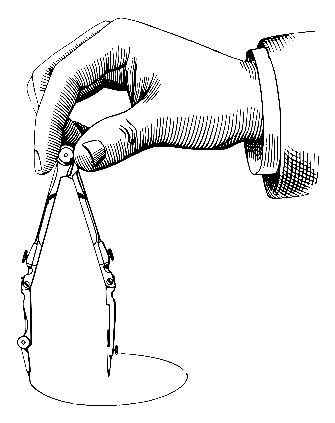
\includegraphics[height=5cm]{./images/compas.eps}
   % compas.eps: 0x0 pixel, 300dpi, 0.00x0.00 cm, bb=
  \end{center}
  \vfill
\end{document}
